\section{Elektrostatische Analyse (ES, Electrostatic Analysis)}
Die elektrostatische Analyse arbeitet mit dem elektrostatischen (ruhenden) Feld. In diesem Fall ist die elektrische Ladung stationär verteilt (Ladungsverteilung ändert sich nicht). Mittels dieser Analyse kann das elektrische Feld, die Kapazität und die Energie in den elektrischen Komponenten berechnet werden.
\subsection{Integralgleichungen}
\begin{tabular}{|p{.30\textwidth} |p{.65\textwidth}|}
	\hline
	\textbf{Gausssches Gesetz}\newline
	{\centering\tabbild[width=4cm]{images/Gauss.png}\par}&
	Der Fluss des Vektors $\vec{D} = \varepsilon\cdot\vec{E}$ durch eine geschlossene orientierte Fläche (A) ist gleich der gesamten elektrischen Ladung Q, die von der Fläche (A) umgeben ist.\newline
	\[\varoiint\limits_{(A)}\vec{D}\cdot\vec{dA} = Q \quad oder \quad \varoiint\limits_{(A)}\vec{E}\cdot\vec{dA} = \dfrac{Q}{\varepsilon}\]
	\[\varoiint\limits_{(A)}\vec{D}\cdot\vec{dA} = Q = \iiint\limits_{(V)}\varrho\cdot dV\]\\
	\hline
	\textbf{Wirbelfreiheit des elektrostatischen Feldes}\newline
	{\centering\tabbild[width=4cm]{images/Wirbelfreiheit}\par}& Das Kurvenintegral des elektrostatischen Feldes $\vec{E}$ über jede geschlossene orientierte Kurve (C) ist gleich null.\newline 
	\[\oint\limits_{(C)}\vec{E}\cdot\vec{dl} = 0\] 
	\[\oint\limits_{(C)}\vec{E}\cdot\vec{dl} = \oint\limits_{\substack{P_1\\ (C_1)} }^{P_2}\vec{E}\cdot\vec{dl} - \oint\limits_{\substack{ P_1\\(C_2)} }^{P_2}\vec{E}\cdot\vec{dl} = 0\]\\
	\hline
	\textbf{Elektrisches Skalarpotential}\newline
	{\centering\tabbild[width = 4cm]{images/Skalarpotential}\par} & Das elektrische Skalarpotential eines Punktes gegenüber dem Bezugspunkt ($P_B$). \newline
	\[\varphi_{P_1} = \oint\limits_{P_1}^{P_N}\vec{E}\cdot\vec{dl}\quad und \quad \varphi_{P_2} = \oint\limits_{P_2}^{P_N}\vec{E}\cdot\vec{dl}\] \[U_{P_1P_2} = \varphi_{P_1} - \varphi_{P_2} = \oint\limits_{P_1}^{P_2}\vec{E}\cdot\vec{dl} \]\\
	\hline	
\end{tabular}
\subsection{Differenzialgleichungen der elektrostatischen Analyse}
\begin{multicols}{2}
	\textbf{Poisson-Gleichung}  \[ \dfrac{\partial^2\varphi}{\partial x^2} +  \dfrac{\partial^2\varphi}{\partial y^2} + \dfrac{\partial^2\varphi}{\partial z^2} =\Delta \varphi = -\dfrac{\rho}{\varepsilon} \]
	\textbf{Gradient} \[ \vec{E}=- \nabla \cdot \varphi = -\gradient \varphi\]
	\textbf{Laplace-Gleichung}  \[ \dfrac{\partial^2\varphi}{\partial x^2} +  \dfrac{\partial^2\varphi}{\partial y^2} + \dfrac{\partial^2\varphi}{\partial z^2} =\Delta \varphi = 0 \]
	\textbf{Divergenz} \[ Q= \nabla \cdot \vec{D}= \divergenz \vec{D} \]
\end{multicols}
\clearpage
\pagebreak
\subsection{Randbedingungen}
\begin{minipage}{8cm}
	\begin{itemize}
		\item Der geerdete Rand \[\varphi = 0\]
		\item Der Rand mit bekannten Potential \[ \varphi = A \]
		\item Der Rand der Symmetrie \[ \dfrac{\partial\varphi}{\partial n} = 0\]
	\end{itemize}
\end{minipage}
\begin{minipage}{8cm}
	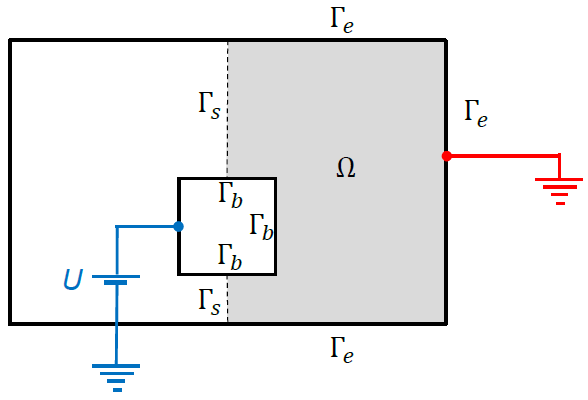
\includegraphics[width=8cm]{images/randbedinung_ES.png}
\end{minipage}
\subsection{Anwendung: pn-Übergang}
Einige Elektronen füllen die Löcher des Gitters und dadurch entsteht eine Raumladungszone. In dieser Zone ist eine Ladung verteilt, aber die Elektronen sind in diesem Bereich nicht frei. 
Durch diese Zone können die Elektronen nicht mehr die Löcher füllen.\\

\[ \varrho_p = \dfrac{Q_p}{d_p\cdot d\cdot L} \] %Gesamte Ladung geteilt durch das Volumen
\[ \varrho_n = \dfrac{Q_n}{d_n\cdot d\cdot L} \] % "

\[\varoiint\limits_{(A)}\vec{E}\cdot\vec{dA} = -\dfrac{\varrho_p}{\varepsilon}\cdot d\cdot L\cdot (x + d_p) \Rightarrow E_{x1}(x) = -\dfrac{\varrho_p}{\varepsilon}\cdot (x + d_p) \]

\[ \varoiint\limits_{(A)}\vec{E}\cdot\vec{n}\cdot \vec{dA} =  \dfrac{Q}{\varepsilon} = \dfrac{\varrho\cdot V}{\varepsilon} = -\dfrac{\varrho_p}{\varepsilon} \]
\clearpage
\pagebreak
